% LaTeX is a simple yet highly dynamic and expandable typesetting language. It is the industry standard for academic writing, scientific and technical documentation, and overall just much more useful than other formats like Microsoft Word, once you get up to speed.

% This document will serve as a baseline lab report template, but also a basic introduction to LaTeX that will serve as a foundation for further learning of the language.

% Firstly, aside from text itself, symbols are the fundamental building blocks in LaTeX. These are the text containers and wrappers distinguished with the backslash (\), and they allow us to manipulate our page and text in an intuitive and direct fashion.

\documentclass{article}
% The document class defines the overall layout. "article" is the standard for short papers and lab reports.

% The area between \documentclass and \begin{document} is called the "Preamble."
% This is where you load packages to add functionality.

\usepackage{geometry} % Allows us to modify page margins and other characteristics.
\geometry{letterpaper, left=20mm, top=20mm, right=20mm, bottom=20mm}

\usepackage{graphicx} % Essential for including images/plots
\usepackage{amsmath}  % The industry standard for formatting math equations
\usepackage{listings} % For including nicely formatted code blocks
\usepackage{xcolor}   % For adding color to code or text
\usepackage{hyperref} % Allows for clickable links and cross-references
% Add this to the preamble
\usepackage{csvsimple}
\usepackage{float}

% Simple setup for code blocks
\lstset{
    basicstyle=\ttfamily\small,
    breaklines=true,
    keywordstyle=\color{blue},
    commentstyle=\color{green!50!black},
    stringstyle=\color{red},
    frame=single
}

\begin{document} % This must be the fist wrapper, and text in here actually gets rendered.
% This is the header. Also, \textbf means text boldface. \textit is italic and \underline is underline, obviously.
\noindent \textbf{Name:} Natalie Poche\\
\textbf{Date:} \today \\ % \today automatically inserts the current date
\textbf{UFID:} 1533-9442

\begin{center} % the begin symbol can also create centered blocks
    \large\textbf{Report - Equipment Demo}
\end{center}

\section{Warm-Up}
Explain the terms volts per div and time per div as applied to an oscilloscope. Where specifically are they indicated on the scope’s display?

Answer: The volts per div are the vertical scale of the oscilloscope. The time per div are the horizontal scale of the oscilloscope. Changes to these values can impact the view of the scope, in otherwords, the zoom in/zoom out portions of the scope.

\section{Warm-Up}
What’s the green terminal on the power supply? What can it be used for and how, physically, could it be used?

Answer: The green terminal on the power supply is the true ground/chassis ground terminal. It can be used when a floating or relative voltage reference is not good enough. It can be physically used by connecting the channel to the circuit's ground node.

\section{Technical}
Explain, in your own words, how the scale settings for voltage & time affect an oscilloscope’s capturing of a waveform. (A good response should identify, describe, and explain the inner workings of an oscilloscope.)

Answer: The scale settings for voltage has two parts. The signal range scale for voltage controls the amplification applied to the input before it reaches the ADC. This determines the ADC's available range and impacts the vertical resolution. The signal range position for voltage impacts the analog front end where it controls the offset DAC that is summed with the input signal. If the signal is positioned too far off-screen, the input can exceed the ADC's range and become clipped, meaning the captured data is actually incorrect rather than merely being displayed incorrectly. The scale settings for time determine the oscilloscope's sampling rate which can impact the resolution of the waveform and the total amount of time included in the capture. A faster time scale allows the oscilloscope to capture rapid changes with greater resolution, while a slower time scale allows a larger time window to be observed.

\section{Scenario}
You are designing a class-D audio amplifier that needs a bipolar, +/-12V DC power supply for the MOSFETs, as well as a 5V DC supply to power to logic circuitry. Make a labelled diagram showing how this could be done with power supplies available in our lab (note: all physical connections should be shown!).

\begin{figure}[H]
    \centering
    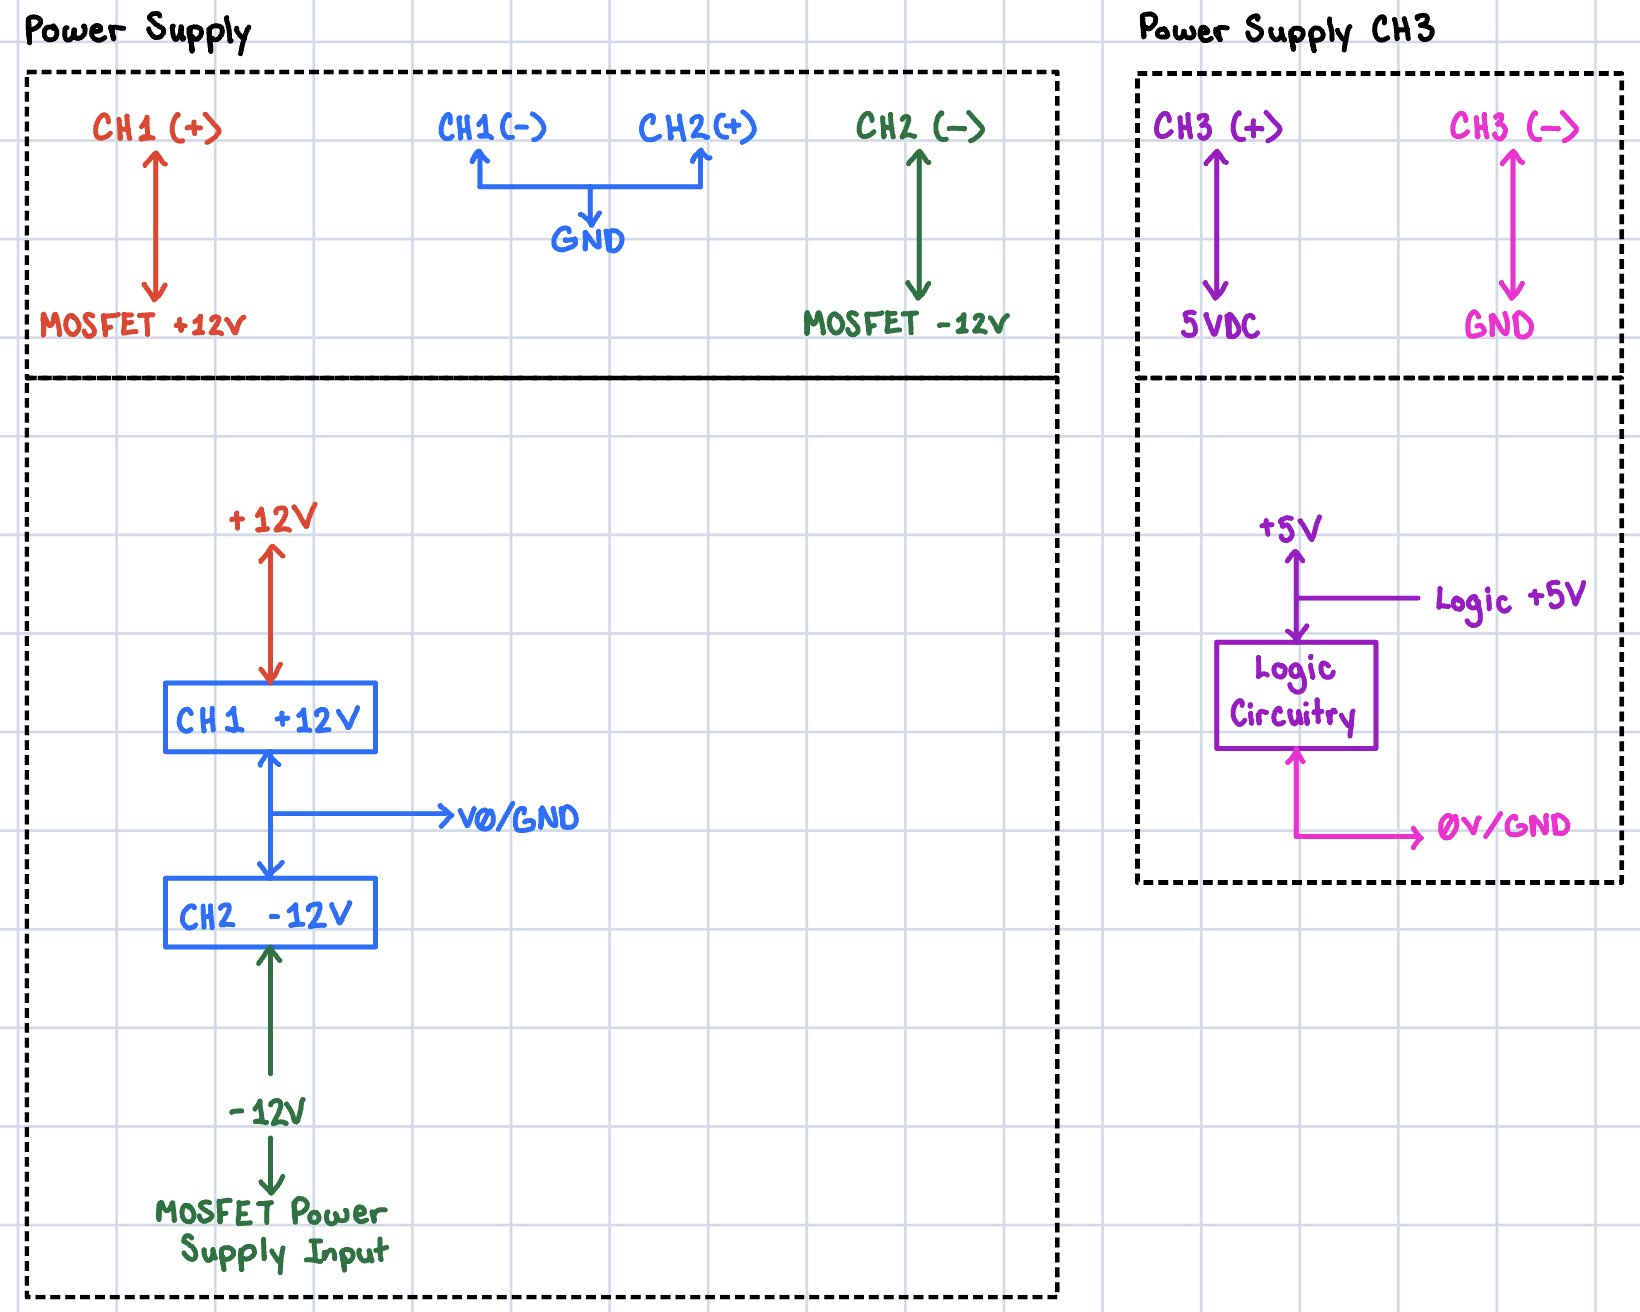
\includegraphics[width=0.6\linewidth]{image0.jpg} % images must be in the same directory for proper compilation. overleaf makes this very simple 
    \caption{Audio Amplifier Diagram (image0.jpg)}
    \label{fig:results} % Labels allow you to reference this figure later (e.g., "As seen in Fig. 1")
\end{figure}

\section{Scenario}
Rob received a synth PCB he designed by mail. He assembled the board and baked it in the reflow oven. He plugged it in and… pop! The power supply was reversed. Oops!!

\subsection{Scenario}
Briefly describe how a programmable power supply and other equipment could detect which component(s) were damaged with minimal risk (hint: faulty components get hot). (Must be practical.)

Answer: A practical approach for Rob would be to use the programmable power supply with a very low current limit then gradually increase the voltage while monitoring the supply current on the board. Look for components that become unusually hot, making sure to turn off if excessive current or rapid heat occurs. Identify the component that gets hot and investigate it for damage. And then repeat the process after replacing the component. 

\subsection{Scenario}
With your help, Rob was able to find and replace the broken parts. He can program his microcontroller, but the SPI interfaced DAC isn’t working as he thinks it should. Briefly describe a technique he could use to debug the circuit.

Answer: A technique to debug the circuit would be to use the oscilloscope to directly observe the SPI signals by probing them. Then by comparing the waveforms and timing to the DAC's datasheet to verify the correct data, chip select, and clock polarity that's being used. This can then indicate whether the problem lies in the firmware or the wiring. If the SPI signals leaving the microcontroller are correct, then the problem is most likely the DAC, the configuring, wiring, or how it's interpreting the received data. If the signals are incorrect, than the issue lies in the microcontroller firmware or SPI configuration. 

\section{Scenario}
You are a test engineer for a drone manufacturer. The flight-ops team describes incidents where drones crash after an aggressive flight maneuver. You think the high motor load during maneuvers is causing the microcontroller to brown out. How could you test this hypothesis?

Answer: First to test it, I would monitor the microcontroller's supply voltage with an oscilloscope while reproducing the aggressive flight maneuver. This would be done by connecting an oscilloscope probe across the microcontroller's supply and ground. Then configuring the oscilloscope to capture the supply voltage. Then reproduce the aggressive maneuver under the controlled conditions. During the maneuver monitor the supply voltage during the period of maximum motor load, and compare the MCU supply voltage during normal operations versus during the aggressive maneuver. Looking for the voltage dip or transient that approaches or falls bellow the microcontroller's minimum operating voltage. If the MCU supply voltage drops below its required operating voltage while the drone is performing the crash prone maneuver, then it would support the brown out hypothesis. 

\section{Practice}
Construct this simple, passive low-pass filter on a breadboard.

\subsection{Practice}
Calculate the theoretical cutoff frequency of this filter. Show your calculations.

Answer: \[f_c = \frac{1}{2\pi RC} = \frac{1}{2*\pi (1000\Omega)(100*10^{-9}F)} = \frac{1}{(2*10{-4}*\pi)} = 1.592kHz\]

\subsection{Practice}
Write a Python script to collect data on the frequency response of the filter. Starting below the cutoff frequency and ending above, use SCPI to iterate the function generator through a series of frequencies and acquire the attenuation from the oscilloscope. Capture at least 32 data points. Save the data in a file and use matplotlib to create a Bode plot for the circuit with (correct) labeled axes, a title, and a marker of the experimental cutoff frequency. The Bode plot should be in the report.

% ============================================================
% Experimental Data Table
% ============================================================

\begin{table}[H]
    \centering
    \caption{Experimental Low-Pass Filter Frequency Response}
    
    \begin{tabular}{|c|c|c|}
        \hline
        Frequency (Hz) & Vout (VPP) & Gain (dB) \\
        \hline
        
        \csvreader[
            head to column names,
            late after line=\\ \hline
        ]{lowpass_data.csv}{}%
        {\csvcoli & \csvcolii & \csvcoliii}
        
    \end{tabular}
    
    \label{tab:lowpass_data}
\end{table}

% image example
% Figures are "floats." LaTeX decides the best place to put them based on any additional directives and the image size. 
% [h] tells LaTeX to put it *h*ere. an exclamation point is to override, so essentially put it here, forced. If you dont distinguish with [h] (or [h!]) or [t] (for top) or any other directions, LaTeX will place the image at the top

\begin{figure}[H]
    \centering
    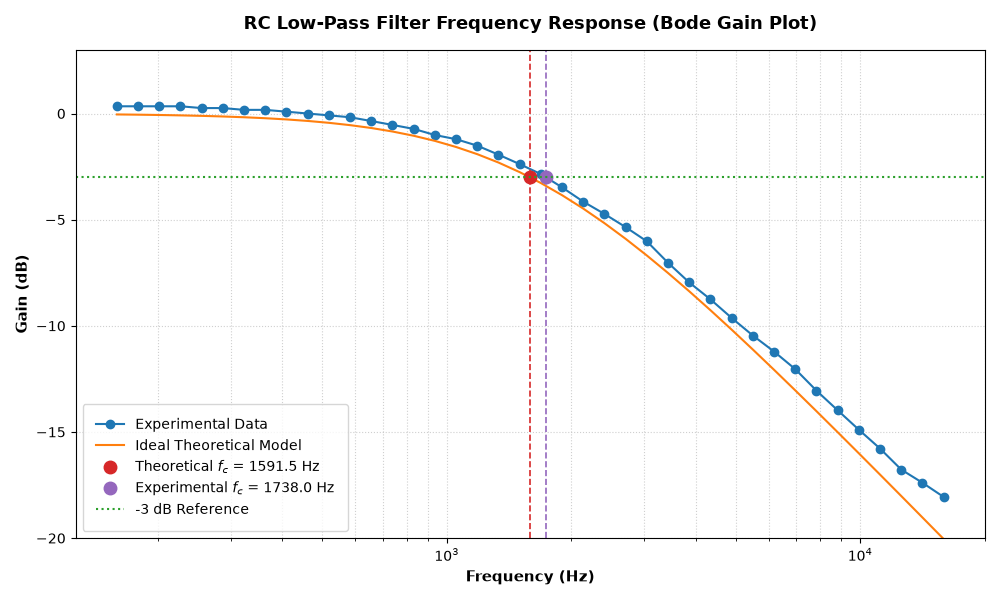
\includegraphics[width=0.6\linewidth]{Figure_1.png} % images must be in the same directory for proper compilation. overleaf makes this very simple 
    \caption{RC Low-Pass Filter Frequency Response Bode Gain Plot (Figure\_1.png)}
    \label{fig:results} % Labels allow you to reference this figure later (e.g., "As seen in Fig. 1")
\end{figure}

\subsection{Practice}
Measure and document the resistor and capacitor values using the multimeter and use the values to calculate the actual cutoff frequency. Does this match the frequency from the Bode plot? If not, what might account for discrepancies?\\\\Capacitor = 107.5 nF\\
Resistor = $1.036 k\Omega$\\
Cutoff Frequency = \[f_c = \frac{1}{2\pi RC} = \frac{1}{2*\pi (1036\Omega)(107.5*10^{-9}F)} = 1.429kHz\] \\\\
While the actual cut off frequency very closely follows the theoretrical expectations, however it does not match the frequency from the Bode plot. This is due to the actual discrepencies in the resistor and capacitor, which were $1.036k\Omega$ and 107.5nF respectively, while the theoretical values were $1k\Omega$ and 100nF respectively. This small differences can be caused from the component tolerances, measurement tool accuracy, or stray resistance and capacitance from the breadboard and wiring. Even though there were some discrepancies, the low pass filter worked as expected. 

% appendix and code
\newpage % Starts a new page for the appendix
\appendix
\section{Scenario}

\lstinputlisting[ language=Python, caption={Python script used to collect the low-pass filter frequency response.}, label={lst:python_code} ]{natalielab01.py}

\end{document}

% Never hesitate to look something up if you need to. LaTeX is used ubiquitously, so chances are, if you can think of some specific functionality, there is probably package for it with documentation or a guide.
